% =============================================================================
% RESULTS THROUGH THE ARCHITECTURE.  Only findings with a mechanism inside a
% block are here; score tables stay in the experiment notes.  Every number is
% quoted from docs/report/insights/experiment_{1,3,4}/experiment_N.tex.
% Finding IDs R1..R13 are stable: the component slides and the index link to
% them by label.
% =============================================================================
\section{Results through the architecture}

\newcommand{\twostrips}[2]{%
  {\centering\adjustbox{scale=0.66}{\parbox{\textwidth}{#1}}\par
   \vspace{-0.15em}\adjustbox{scale=0.66}{\parbox{\textwidth}{#2}}\par}\vspace{0.1em}}

% ---------------------------------------------------------------- map
\begin{frame}{2.0 \;Where the results land}
  \centering\scriptsize
  Each finding below is a place where a result can be explained by one block.
  Click an R-number to jump.\par\vspace{0.4em}
  \adjustbox{max width=\textwidth}{%
  \begin{tabular}{@{}l l l@{\qquad}l l l@{}}
    \toprule
    & Block & Finding & & Block & Finding \\
    \midrule
    \hyperlink{R1}{\textbf{R1}} & ORB-1 & faster front end, same accuracy &
    \hyperlink{R8}{\textbf{R8}} & ORB-1/2, VINS-1/2 & real rig: better images, slower robot \\
    \hyperlink{R2}{\textbf{R2}} & ORB-7, ORB-8 & false loop closure on a repeated object &
    \hyperlink{R9}{\textbf{R9}} & ORB-1, 5, 6 & three rules for reading ORB numbers \\
    \hyperlink{R3}{\textbf{R3}} & ORB-6, ORB-8 & gravity needs a turn; tilt becomes height &
    \hyperlink{R10}{\textbf{R10}} & RTAB-5, RTAB-6 & words propose, geometry disposes \\
    \hyperlink{R4}{\textbf{R4}} & ORB-6 & a robot standing still resets the map &
    \hyperlink{R11}{\textbf{R11}} & RTAB-3/8/9, NAV-2 & the first second poisons two layers \\
    \hyperlink{R5}{\textbf{R5}} & VINS-1 vs ORB-3 & blank wall: VINS starves, ORB bridges &
    \hyperlink{R12}{\textbf{R12}} & RTAB-8 $\rightarrow$ NAV-3 & poses are fine, the grid is not \\
    \hyperlink{R6}{\textbf{R6}} & VINS-1, VINS-4 & fisheye rim: dividing by $z$ explodes &
    \hyperlink{R13}{\textbf{R13}} & RTAB-9 & the pose is as good as the map \\
    \hyperlink{R7}{\textbf{R7}} & ORB-3, VINS-1/4 & the one mover that hurts: ahead, same way &
    \hyperlink{R14}{\textbf{R14}} & Nav2, \ldots & what is not measured yet \\
    \bottomrule
  \end{tabular}}
  \par\vspace{0.6em}
  \begin{tabular}{@{}l@{\quad}l@{}}
    \textbf{Experiment 1} & localisation accuracy: ORB-SLAM3 vs VINS-Fusion, sim (4 bags) and real rig (realv6/7) \\
    \textbf{Experiment 3} & map quality: RTAB-Map occupancy grid against the world \\
    \textbf{Experiment 4} & relocalisation in a prior map: RTAB-Map + ORB-SLAM3, 6 hand-driven runs \\
  \end{tabular}
\end{frame}

% ---------------------------------------------------------------- R1
\begin{frame}[label=R1]{R1 \;ORB-1 \;A faster front end buys frames, not accuracy}
  \hl{ORB1}\orbstrip\par\vspace{0.2em}
  \finding{orbc}{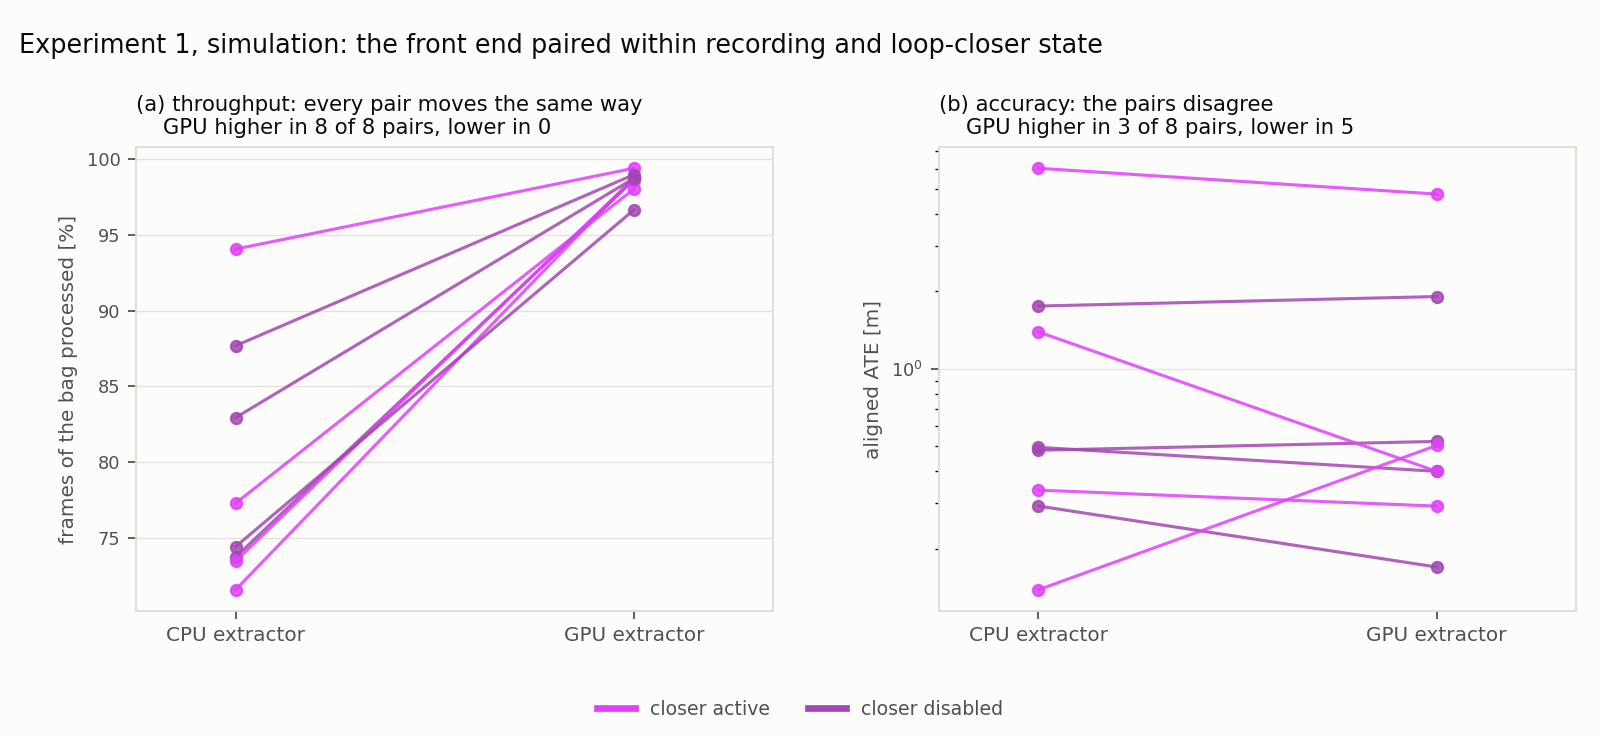
\includegraphics{exp1_frontend_pairs.png}}%
  {Swap only the extractor (CPU $\rightarrow$ GPU), same bag, same closer state.
   \textbf{Sim:} frames kept rise in 8 of 8 pairs (72--94\,\% $\rightarrow$ 97--99\,\%);
   ATE rises in 3, falls in 5.
   \textbf{Robot:} 6 of 6 pairs, ATE within 0.02\,m.}%
  {ORB-1 only decides how many frames reach ORB-3. The robot moves
   0.28\,m/s, so even the CPU's 9\,Hz is 3\,cm per frame: nothing is missed.
   The large errors come from discrete events further down the chain
   (\R{2}{}, \R{3}{}).}%
  {one run per cell; ORB-SLAM3 repeats spread up to 0.28\,m (\R{9}{}), wider than most gaps.}
\end{frame}

% ---------------------------------------------------------------- R2
\begin{frame}[label=R2]{R2 \;ORB-7 + ORB-8 \;A false loop closure on a repeated object}
  \hl{ORB7}\hl{ORB8}\orbstrip\par\vspace{0.2em}
  \finding{orbc}{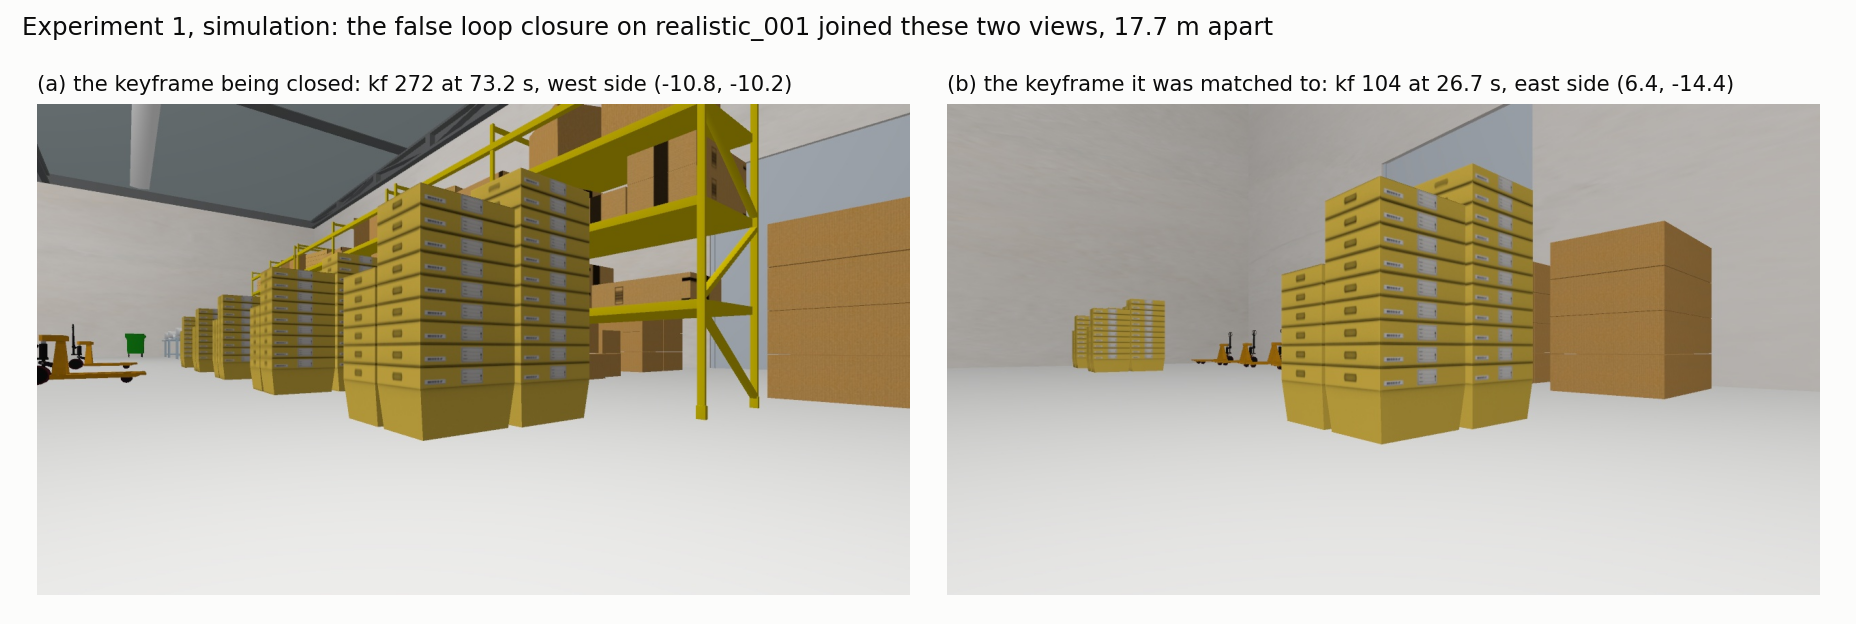
\includegraphics{exp1_false_closure.png}}%
  {Static I layout, \textbf{73.2\,s}: both front ends accept one closure,
   correction 14.7\,m (CPU) / 13.3\,m (GPU). The run ends 6.0 / 4.8\,m off;
   with the closer off: 0.50 / 0.40\,m.
   \textbf{Robot:} one loop-closing repeat took a \textbf{36.4\,m} closure, ended 10.7\,m off.}%
  {ORB-7 matched two keyframes 17.7\,m apart: same box-stack, so same
   words, and the geometric check passes because the objects
   \emph{are} identical. ORB-8 then bends the whole map. Nothing asks whether
   14\,m is plausible after 0.5\,m of drift.}%
  {diagnosed, not fixed. A correction bound like our RTAB-9 gate (\R{13}{}) is untested on ORB-8.}
\end{frame}

% ---------------------------------------------------------------- R3
\begin{frame}[label=R3]{R3 \;ORB-6 \;Gravity is found only while the robot turns}
  \hl{ORB6}\hl{ORB8}\orbstrip\par\vspace{0.2em}
  \finding{orbc}{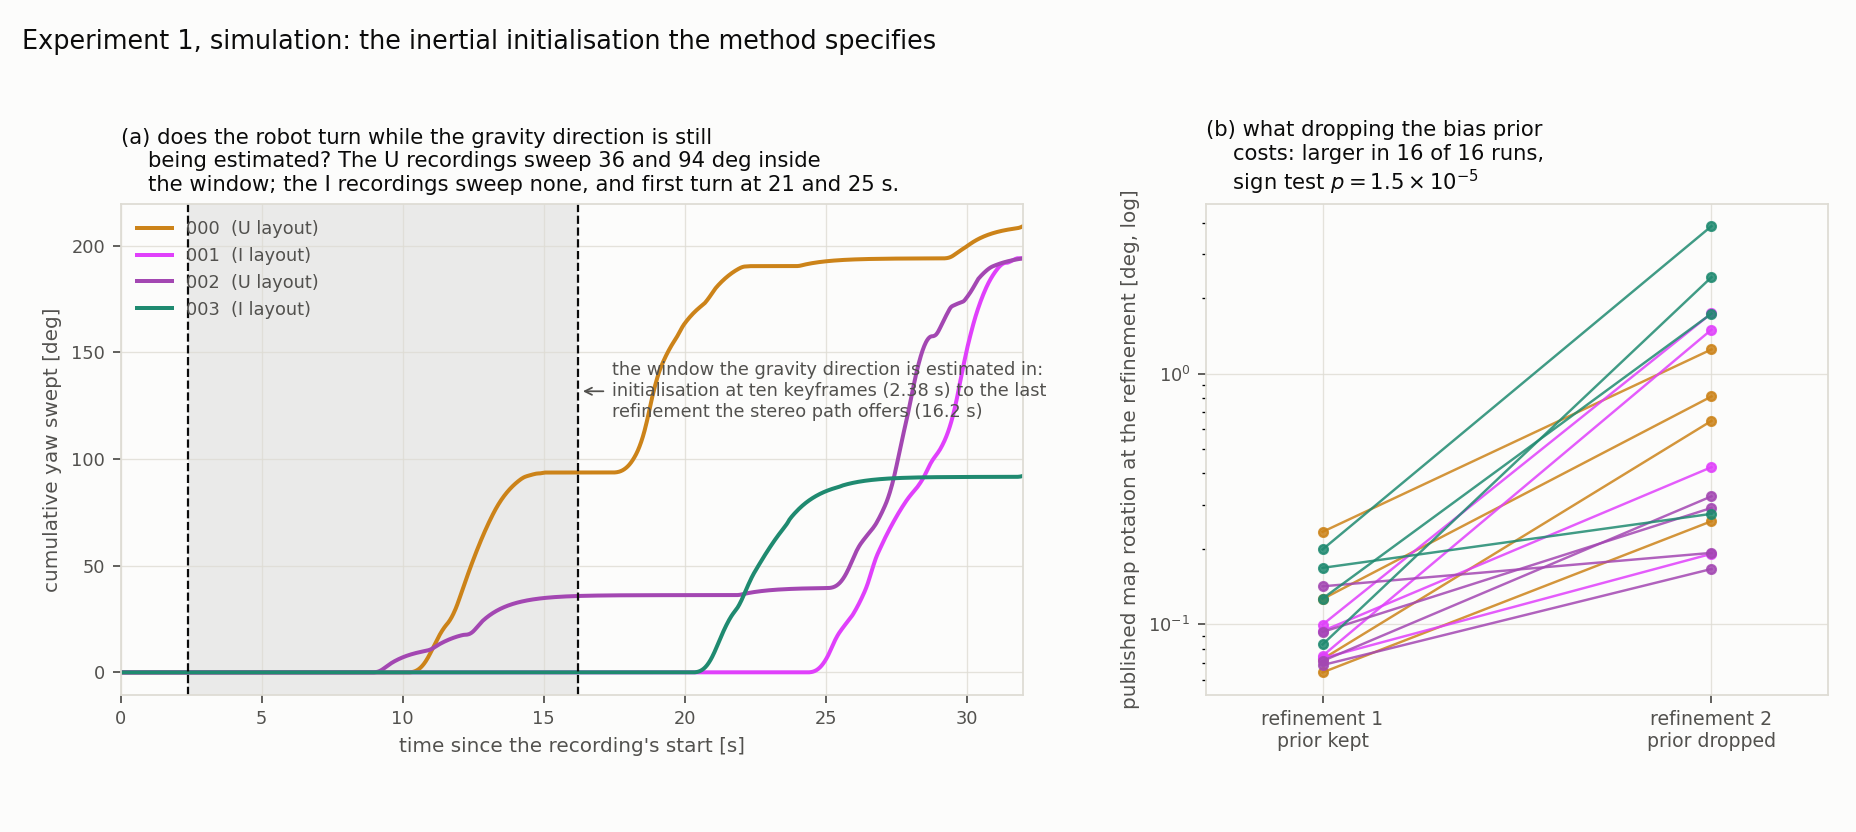
\includegraphics{exp1_imu_init.png}}%
  {In the init window (2.4--16.2\,s) the U routes turn 36--94$^\circ$, the I
   routes \textbf{0$^\circ$}. Tilt left over: 0.24--0.72$^\circ$ (U) vs
   up to 3.7$^\circ$ (I). On the I traffic bag the closer-off runs climb
   4.7--5.1\,m; with the closer on, 0.6--1.4\,m.}%
  {ORB-6 solves gravity direction and accelerometer bias together; they
   separate only if the body rotates. Drive straight for 16\,s and gravity
   stays tilted, with no later re-estimate on the stereo path. A tilted floor
   turns distance into height. Only a closure (ORB-8) pulls it back.}%
  {layout and opening move are confounded (2 routes vs 2). Test: an I-layout bag that turns in its first 15\,s.}
\end{frame}

% ---------------------------------------------------------------- R4
\begin{frame}[label=R4]{R4 \;ORB-6 \;A robot standing still at the start resets the map}
  \hl{ORB6}\orbstrip\par\vspace{0.2em}
  \finding{orbc}{%
  \begin{tikzpicture}[font=\scriptsize]
    \fill[offc!35] (0,-0.55) rectangle (2.2,-0.1); \node at (1.1,-0.33) {standing still};
    \draw[-{Latex}] (0,0) -- (8.6,0) node[right]{t};
    \draw[orbc, very thick] (1.0,-0.1) -- (1.0,0.35) node[above, text=orbc]{IMU init $\sim$3\,s};
    \draw[decorate, decoration={brace, amplitude=3pt, mirror}] (1.0,-0.7) -- (5.0,-0.7)
      node[midway, below=4pt]{10\,s check: keyframes moved $<$ 2\,cm?};
    \node[draw=bad, thick, rounded corners, align=center, fill=bad!8] (rs) at (3.3,1.7)
      {upstream:\\map \textbf{reset}};
    \draw[arr, bad] (2.0,0.05) -- (rs);
    \node[draw=bad, thick, rounded corners, align=center, fill=bad!8] (re) at (6.9,1.7)
      {re-init waits for an\\\textbf{empty} keyframe queue\\$\Rightarrow$ never (1 KF / 0.25\,s)};
    \draw[arr, bad] (rs) -- (re);
    \node[draw=good, thick, rounded corners, align=center, fill=good!8] at (4.3,-2.0)
      {patch 15: init with a backlog $\cdot$ no low-motion reset for stereo};
  \end{tikzpicture}}%
  {Robot recordings realv7, upstream: the IMU stayed uninitialised for most
   of 9 of 12 runs. With patch 15: IMU initialises at 2.8--4.7\,s in every
   run; 13 of 16 runs need no reset; floor tilt 0.2--2.8$^\circ$.}%
  {The upstream rule is written for hand-held cameras that move from the
   first second. A robot waiting at its start pose satisfies ``too little
   motion'' and gets reset; the re-try then starves behind ORB-5's
   keyframe queue.}%
  {patch 15 makes the runs scorable; it does \emph{not} make them more accurate (matches / splits / wins over three bags).}
\end{frame}

% ---------------------------------------------------------------- R5
\begin{frame}[label=R5]{R5 \;VINS-1 vs ORB-3 \;At a blank wall VINS starves and ORB bridges}
  \hl{VINS1}\hl{VINS4}\hl{ORB2}\hl{ORB3}\twostrips{\vinsstrip}{\orbstrip}
  \finding{vinsc}{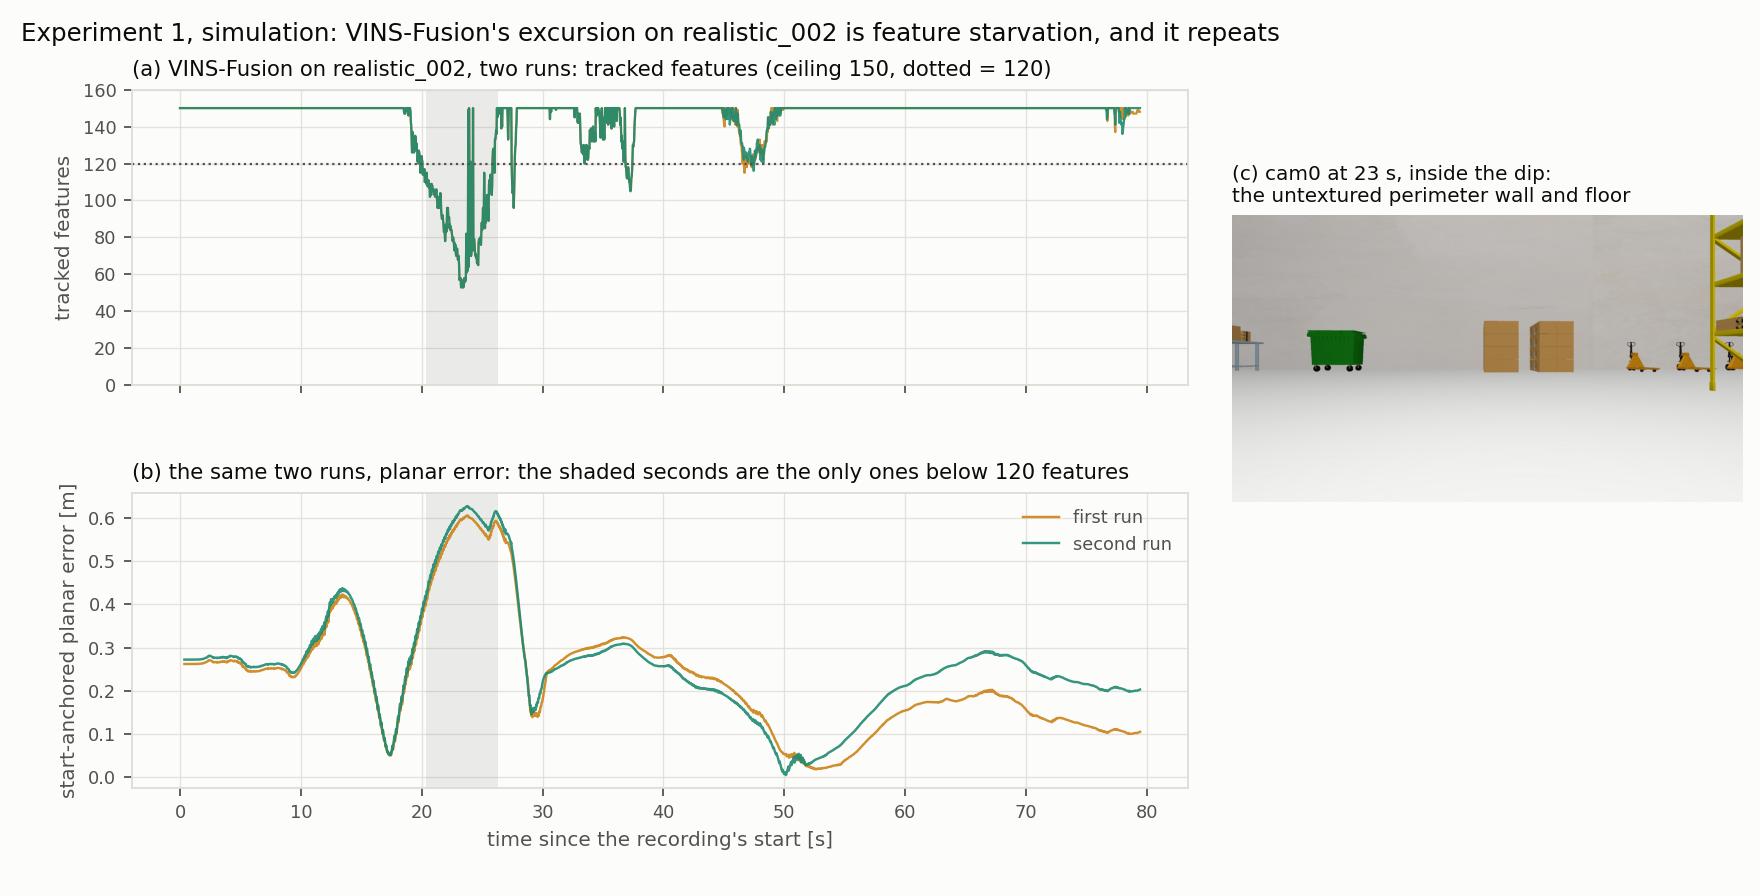
\includegraphics{exp1_vins_starvation.png}}%
  {U traffic bag, east aisle, 20--26\,s: VINS features 150 $\rightarrow$
   \textbf{53}, error +0.18\,m. A repeat run gives the same dip in the same
   second, within 6\,mm. ORB at a blank wall: 500 $\rightarrow$ $\sim$110 points
   for under 1\,s, no step.}%
  {VINS-1 can only keep corners that exist; blank wall + blank floor leave
   nothing to follow for 7\,s, and VINS-4 drifts. ORB-3 passes the same kind
   of wall in one second because ORB-2's IMU prediction carries it. Stereo
   depth held (92\,\%): it is the tracker, not the depth.}%
  {low-feature seconds are 8--20\,\% of a run: this explains VINS's \emph{excursions}, not its ATE. It cannot happen on the robot (\R{8}{}).}
\end{frame}

% ---------------------------------------------------------------- R6
\begin{frame}[label=R6]{R6 \;VINS-1 \;On a fisheye, dividing by depth explodes at the rim}
  \hl{VINS1}\hl{VINS4}\vinsstrip\par\vspace{0.2em}
  \finding{vinsc}{%
  \begin{tikzpicture}[font=\scriptsize, x=0.055cm, y=0.32cm]
    \draw[-{Latex}] (0,0) -- (100,0);
    \node at (50,-2.0) {ray angle $\theta$ from the optical axis ($^\circ$)};
    \draw[-{Latex}] (0,0) -- (0,13);
    \node[anchor=south west] at (2,13) {lifted $x/z = \tan\theta$};
    \foreach \t in {0,30,60,90} \draw (\t,0.15) -- (\t,-0.15) node[below]{\t};
    \fill[bad!12] (70,0) rectangle (90,12.5);
    \draw[very thick, vinsc, domain=0:85.3, samples=80] plot (\x,{tan(\x)});
    \draw[dashed, good, thick] (70,0) -- (70,12.5) node[above, text=good]{mask 70$^\circ$};
    \draw[dashed, black!50] (90,0) -- (90,12.5);
    \node[text=bad, align=center] at (80,7) {26\,\% of\\corners\\cut};
    \node[align=left, text=black!70, anchor=west] at (8,10.5) {fisheye: corners reach\\the lens rim ($\sim$90$^\circ$)};
  \end{tikzpicture}}%
  {Robot, before the fix: VINS diverged on every recording, to $10^8$\,m on
   realv7\_001 (``parallax'' 6\,740\,px). After: three valid runs,
   0.37--0.68\,m, no reset; still 1.6--1.9$\times$ behind ORB.}%
  {VINS-1 turns each point into $(x/z,\,y/z)$. Near 90$^\circ$, $z\!\to\!0$: a
   corner on the rim lands thousands of units out and poisons VINS-4. Second
   fault: \texttt{estimate\_extrinsic} 1 let VINS-4 ``refine'' the stereo
   baseline away; now 0.}%
  {ORB uses the same lens model but never divides by $z$. The model also stops being monotonic at 109.3$^\circ$: real, but that band is black.}
\end{frame}

% ---------------------------------------------------------------- R7
\begin{frame}[label=R7]{R7 \;ORB-3 + VINS-1 \;The one mover that hurts: close, ahead, same way}
  \hl{ORB3}\hl{VINS1}\hl{VINS4}\twostrips{\orbstrip}{\vinsstrip}
  \finding{orbc}{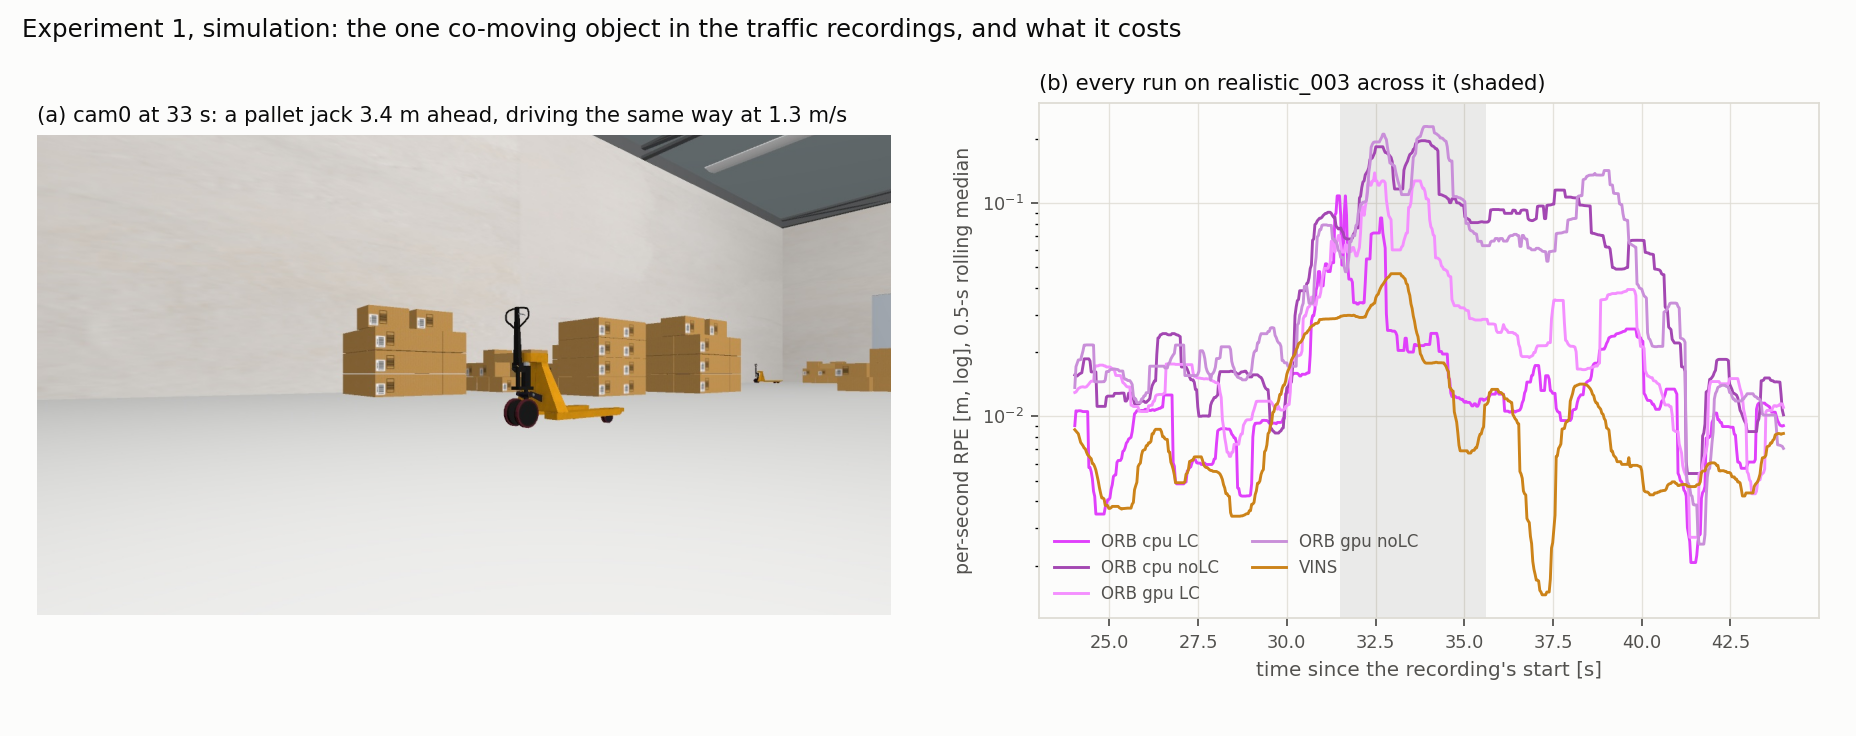
\includegraphics{exp1_jack_ahead.png}}%
  {I traffic bag, 31.5--35.6\,s: a pallet jack 3.4\,m ahead at 1.3\,m/s, the
   robot at 1.56. Error per second $\times$2--7.7 (ORB), $\times$3 (VINS);
   total step only $-0.03$ to $+0.09$\,m. Movers merely in view or crossing:
   \textbf{no cost}.}%
  {ORB-3 and VINS-4 drop points whose reprojection disagrees with the
   estimated motion (VINS-1's F-test is off in our fork). A co-moving object
   barely moves in the image, so its points pass as static structure.
   6--20\,m away the same jack did nothing.}%
  {one 4-second episode in 117\,s. Supports the project hypothesis in this one case, not ``movers degrade the estimate'' in general.}
\end{frame}

% ---------------------------------------------------------------- R8
\begin{frame}[label=R8]{R8 \;ORB-1/2 + VINS-1/2 \;Real rig: better images, slower robot}
  \hl{ORB1}\hl{ORB2}\hl{VINS1}\hl{VINS2}\twostrips{\orbstrip}{\vinsstrip}
  \finding{sysc}{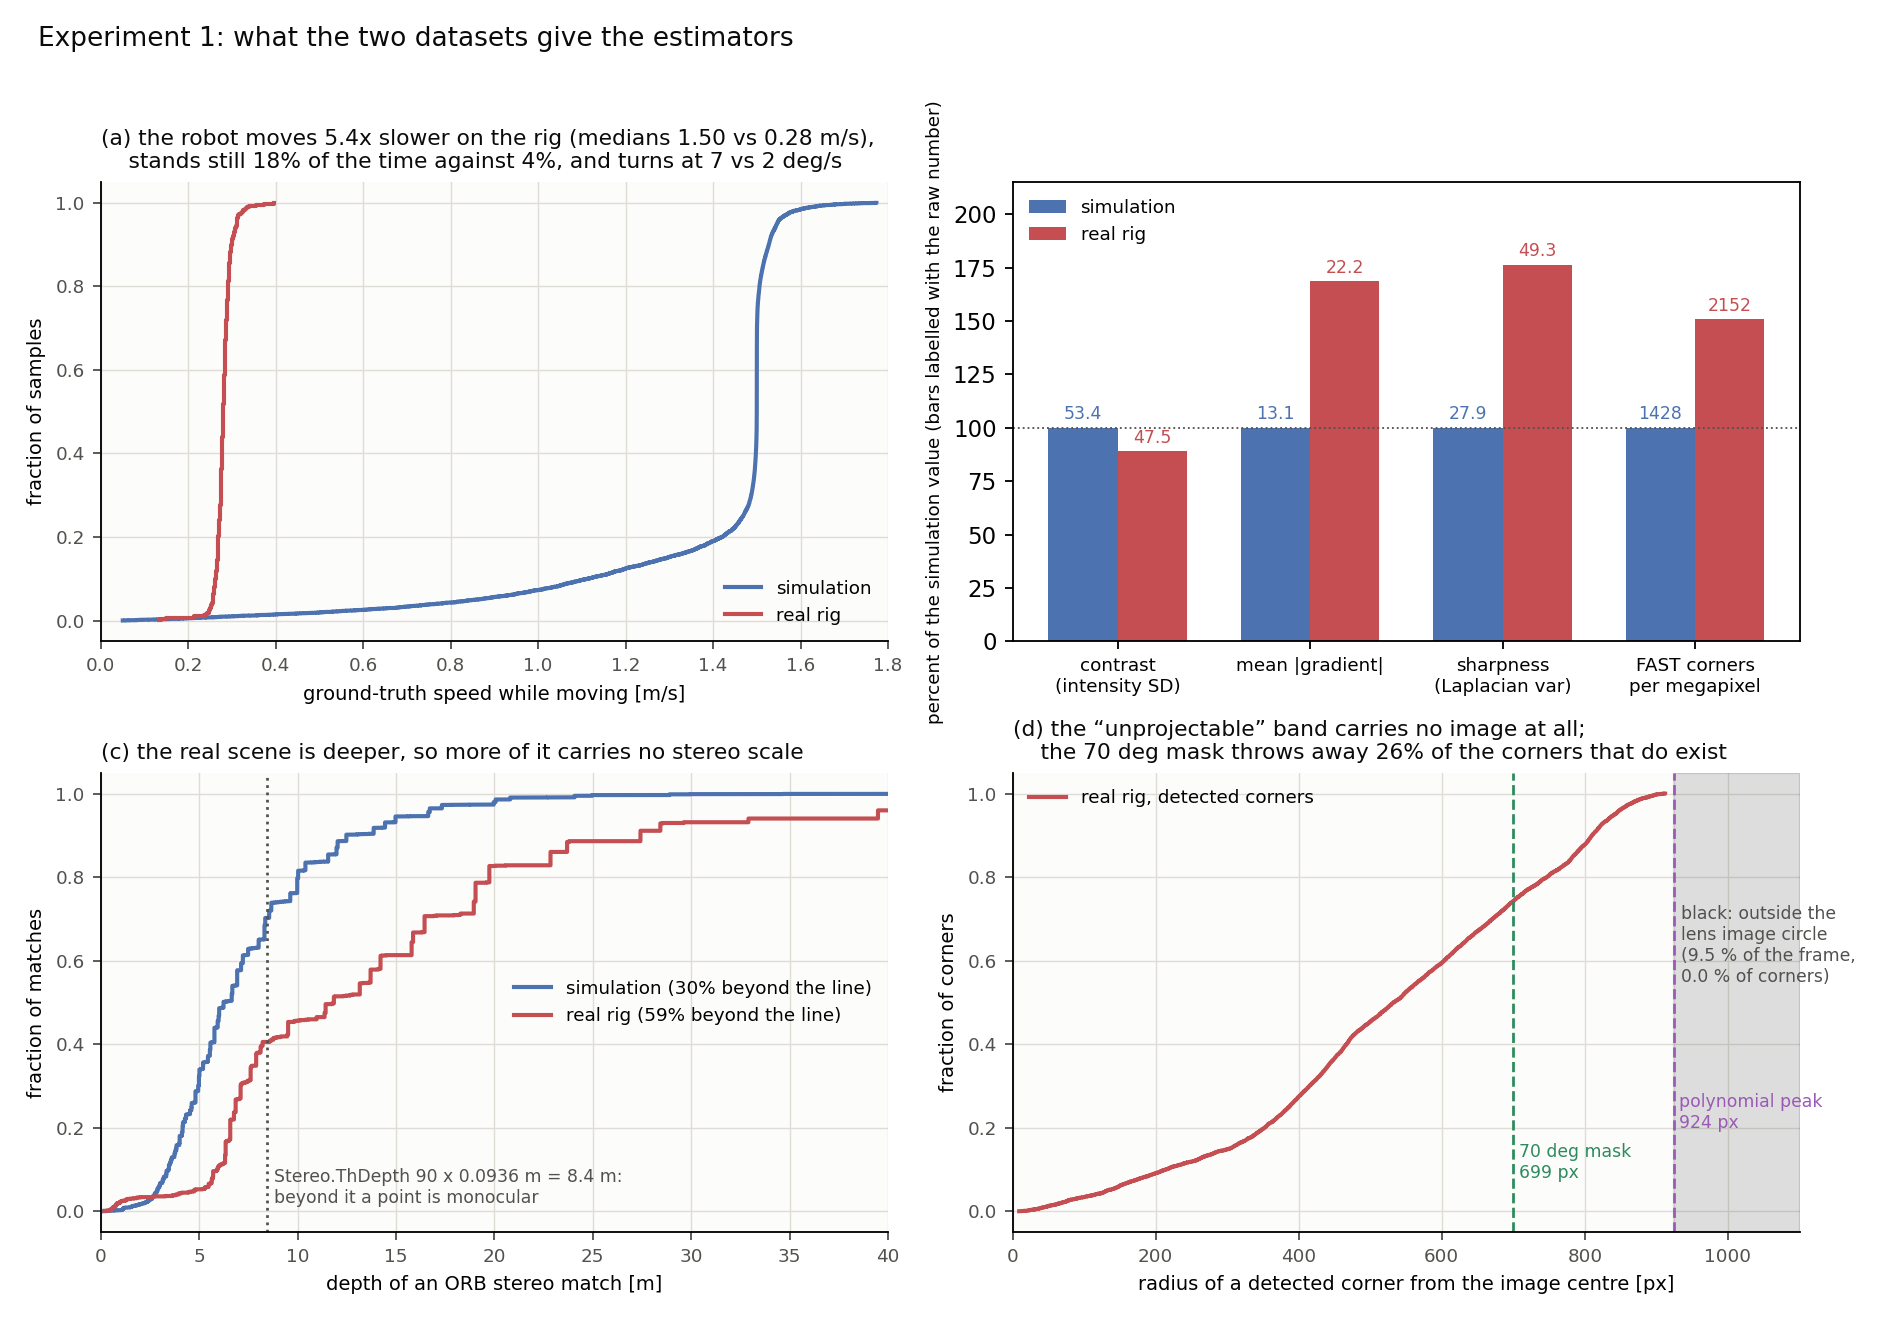
\includegraphics{exp1_dataset_compare.png}}%
  {Real frames: 169\,\% of sim gradient, \textbf{3$\times$} corners per frame;
   VINS holds 150 features 100\,\% of seconds. But 0.28 vs 1.50\,m/s
   $\Rightarrow$ \textbf{5.8$\times$} more IMU time per metre. 59\,\% of stereo
   matches beyond 8.4\,m (sim 30\,\%). Drift: 1.9$\times$ per second,
   10.5$\times$ per metre.}%
  {ORB-1 / VINS-1 have more corners than they use, so detection is not the
   limit. ORB-2 / VINS-2 integrate per \emph{second}: bias, gravity tilt and
   standing still all grow with time. ThDepth 90 $\times$ 0.0936\,m = 8.4\,m:
   beyond it ORB-1 stereo gives direction but no scale.}%
  {compare the two domains per second, never per metre.}
\end{frame}

% ---------------------------------------------------------------- R9
\begin{frame}[label=R9]{R9 \;ORB-1, 5, 6 \;Three rules for reading an ORB-SLAM3 number}
  \hl{ORB1}\hl{ORB5}\hl{ORB6}\orbstrip\par\vspace{0.6em}
  \centering\small
  \begin{tabular}{@{}p{0.27\textwidth} p{0.33\textwidth} p{0.33\textwidth}@{}}
    \toprule
    \textbf{Rule} & \textbf{Measured} & \textbf{Block behind it} \\
    \midrule
    1. Differences under \textbf{$\sim$0.25\,m} are noise &
    3 identical repeats: ORB spreads up to 0.277\,m (80\,\% of its mean); VINS 3--7\,\% &
    ORB-1 drops different frames each run (70--98\,\% kept), ORB-5 runs on its own thread; VINS took every frame \\
    \addlinespace
    2. Score rotation \textbf{after} the 90$^\circ$ step &
    rotation RMS 13--19$^\circ$, median 0.25--2.5$^\circ$ &
    ORB-6 switches the published frame from camera to gravity at init: a convention, not an error \\
    \addlinespace
    3. A path 2--5\,\% too long is \textbf{not} a scale error &
    after init: 0.997--0.999 local scale &
    the arc length of the pre-init spike (3--8\,m in the first 3.5\,s) \\
    \bottomrule
  \end{tabular}
  \src{Experiment 1 note: ``How repeatable is any of this?'', ``the rotation column'', ``the path excess is not a scale bias''.}
\end{frame}

% ---------------------------------------------------------------- R10
\begin{frame}[label=R10]{R10 \;RTAB-5 + RTAB-6 \;The words propose, the geometry disposes}
  \hl{RTAB5}\hl{RTAB6}\rtabstrip\par\vspace{0.2em}
  \finding{rtabc}{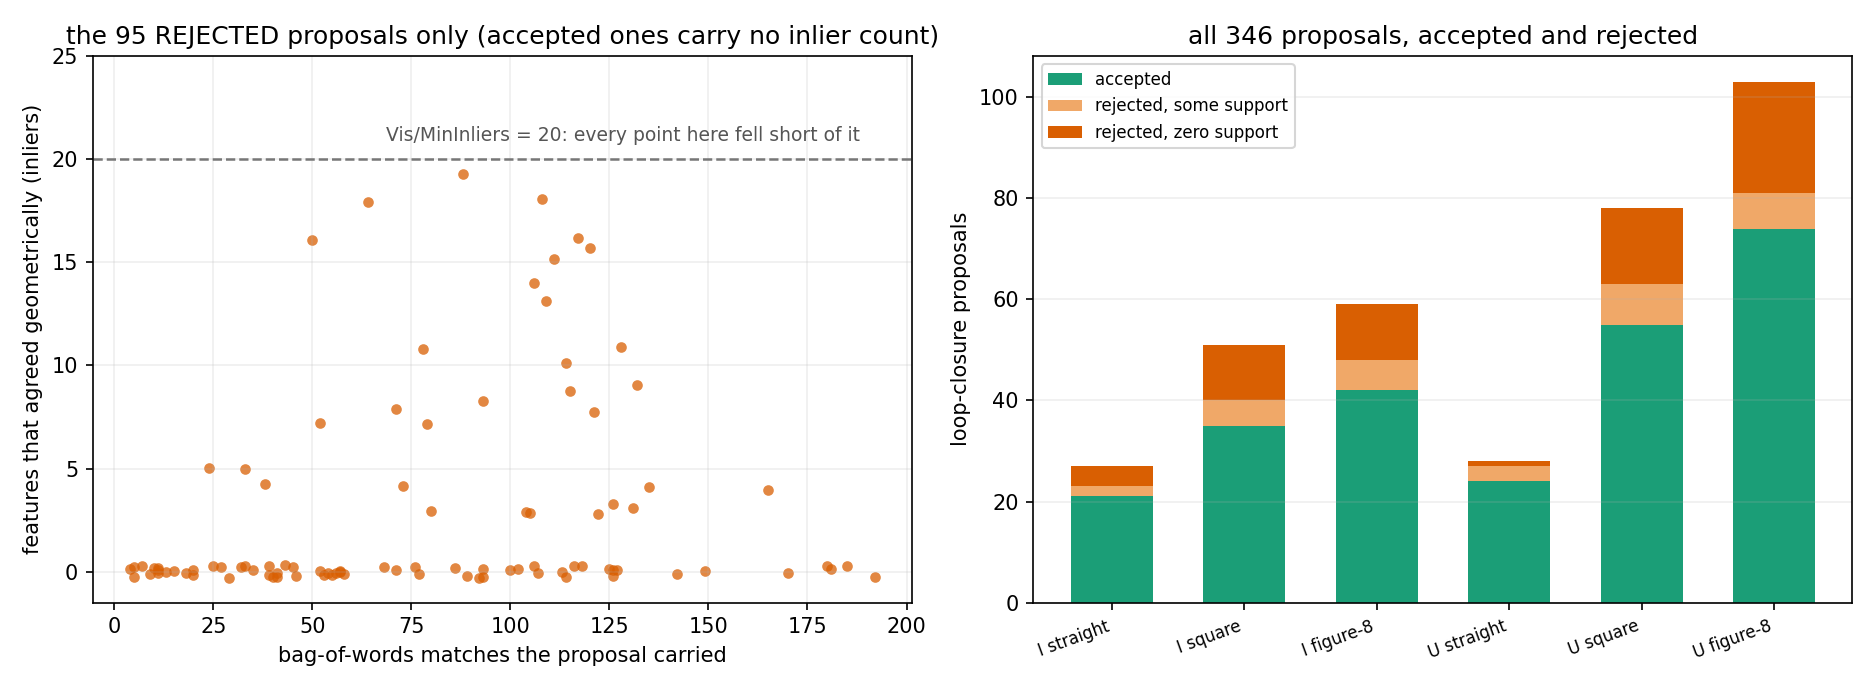
\includegraphics{exp4_rtabmap_gating.png}}%
  {6 relocalisation runs: 346 proposals, 251 accepted (73\,\%). Of the 95
   rejected, \textbf{64 had zero} features agreeing in metres, carrying a
   median of 77 matching words and up to 192.}%
  {RTAB-5 votes on shared words, and repeated rack faces give two aisles
   about 100 words in common. RTAB-6 checks in metres (MinInliers 20) and
   throws them out. This is the aliasing of \R{2}{}, caught here.
   MinInliers 35 stopped the warping but one bag then localised on 0 of 81
   poses.}%
  {inlier counts are logged only for rejections, so accepted proposals cannot be compared.}
\end{frame}

% ---------------------------------------------------------------- R11
\begin{frame}[label=R11]{R11 \;RTAB-3/8/9 + NAV-2 \;The first second poisons two layers}
  \hl{RTAB3}\hl{RTAB8}\hl{RTAB9}\rtabstrip\par\vspace{0.2em}
  \finding{rtabc}{%
  \begin{tikzpicture}[font=\scriptsize]
    \fill[bad!20] (0,0.02) rectangle (1.0,0.45); \node[text=bad] at (0.5,0.24) {1\,s};
    \draw[-{Latex}] (0,0) -- (9.4,0) node[right]{t};
    \node[anchor=north west, align=left] at (-0.1,-0.15) {front-end orientation\\still settling (ORB-6)};
    \node[box, text width=38mm, fill=mapcol!8] (map) at (2.2,2.5)
      {\textbf{mapping} (RTAB-3/8): the first 5 nodes lay phantom cells at the spawn};
    \node[box, text width=38mm, fill=mapcol!8] (loc) at (7.0,2.5)
      {\textbf{localise} (RTAB-9): a fix taken now latches a 73--76$^\circ$ wrong correction for $\sim$16\,s};
    \draw[arr, bad] (0.4,0.45) -- (map.south -| 0.4,0);
    \draw[arr, bad] (0.8,0.45) to[out=30, in=-100] (loc.south);
    \draw[good, very thick] (5.0,-0.2) -- (5.0,0.35);
    \node[text=good, anchor=north] at (5.0,-0.25) {\texttt{localize\_delay\_s} = 5\,s};
  \end{tikzpicture}}%
  {Localise: holding RTAB-Map back 5\,s cut the largest correction yaw from
   110--177$^\circ$ to 25$^\circ$ (3 runs). Map: 63--96\,\% of the phantom cells
   that block the spawn area came from the first five nodes.}%
  {Both layers consume the same unstable second. \texttt{wait\_for\_imu\_init}
   does not help (the flag is already true), and NAV-2's
   \texttt{init\_ignore\_s} acts only after the correction is formed.
   One rule for both: \textbf{do not consume the first second.}}%
  {the map-side fix (drop the first nodes' cells) is predicted by the data, not yet tested.}
\end{frame}

% ---------------------------------------------------------------- R12
\begin{frame}[label=R12]{R12 \;RTAB-8 $\rightarrow$ NAV-3 \;The poses are right, the grid is not}
  \hl{RTAB8}\hl{NAV3}\twostrips{\rtabstrip}{\navstrip}
  \finding{rtabc}{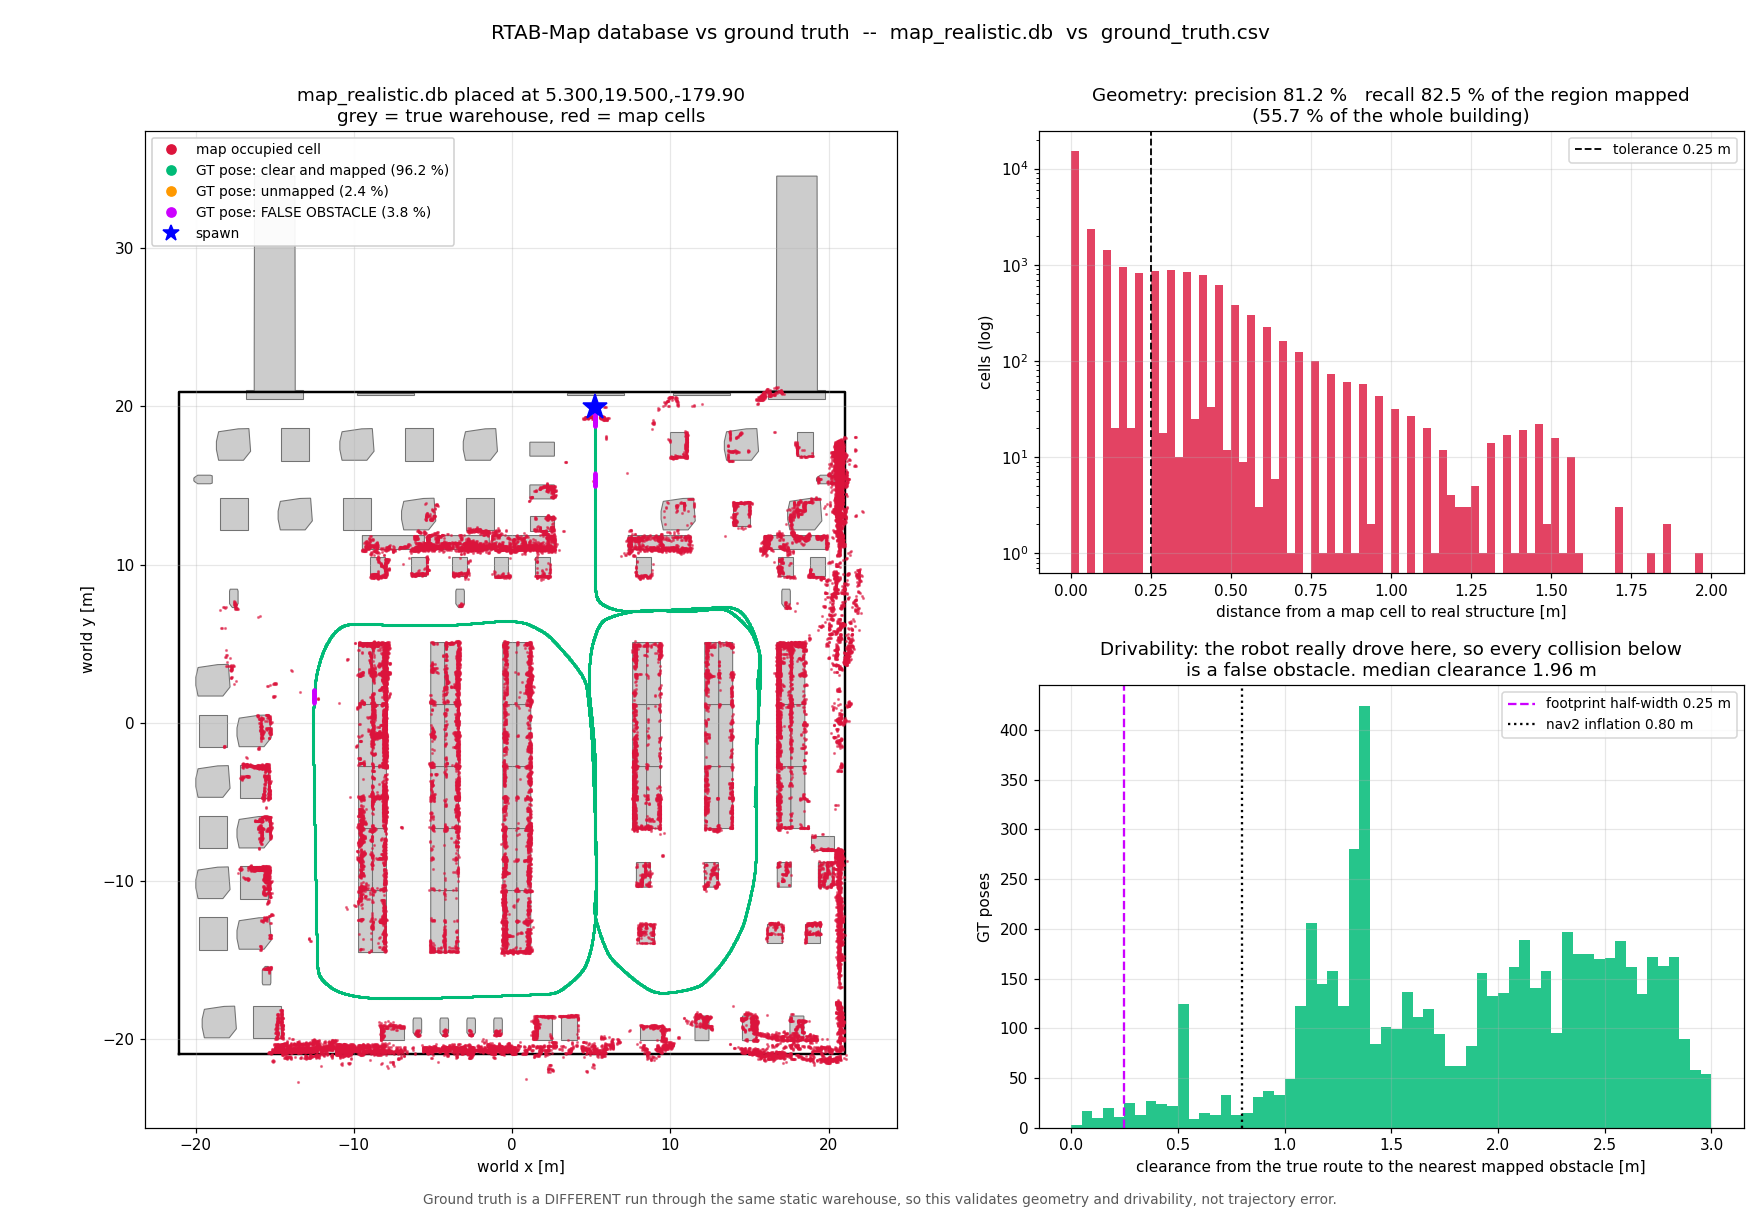
\includegraphics{map_realistic_validate.png}}%
  {4 closure-free maps. Graph poses \textbf{0.10--0.40\,m} rms over
   365--381\,m; a best fit improves them by $\le$\,0.012\,m. Grid precision
   77.8--84.8\,\% (target 90), false obstacles \textbf{3.8--10.2\,\%} (target 1):
   thickened shelves, walls $\sim$0.5\,m off, spawn phantoms.}%
  {The loss is made in RTAB-8, where depth images become cells
   (\texttt{Grid/RangeMax}, \texttt{MaxGroundHeight}, ray tracing), not in
   the trajectory. NAV-3 reads this \texttt{/map} with
   \texttt{allow\_unknown} false and 0.80\,m inflation: a phantom becomes a
   wall the planner must respect.}%
  {I-layout graphs have a 2.6--3.2\,m worst node; builds A/B changed 3 parameters at once.}
\end{frame}

% ---------------------------------------------------------------- R13
\begin{frame}[label=R13]{R13 \;RTAB-9 \;The pose is as good as the map behind it}
  \hl{RTAB9}\rtabstrip\par\vspace{0.2em}
  \finding{rtabc}{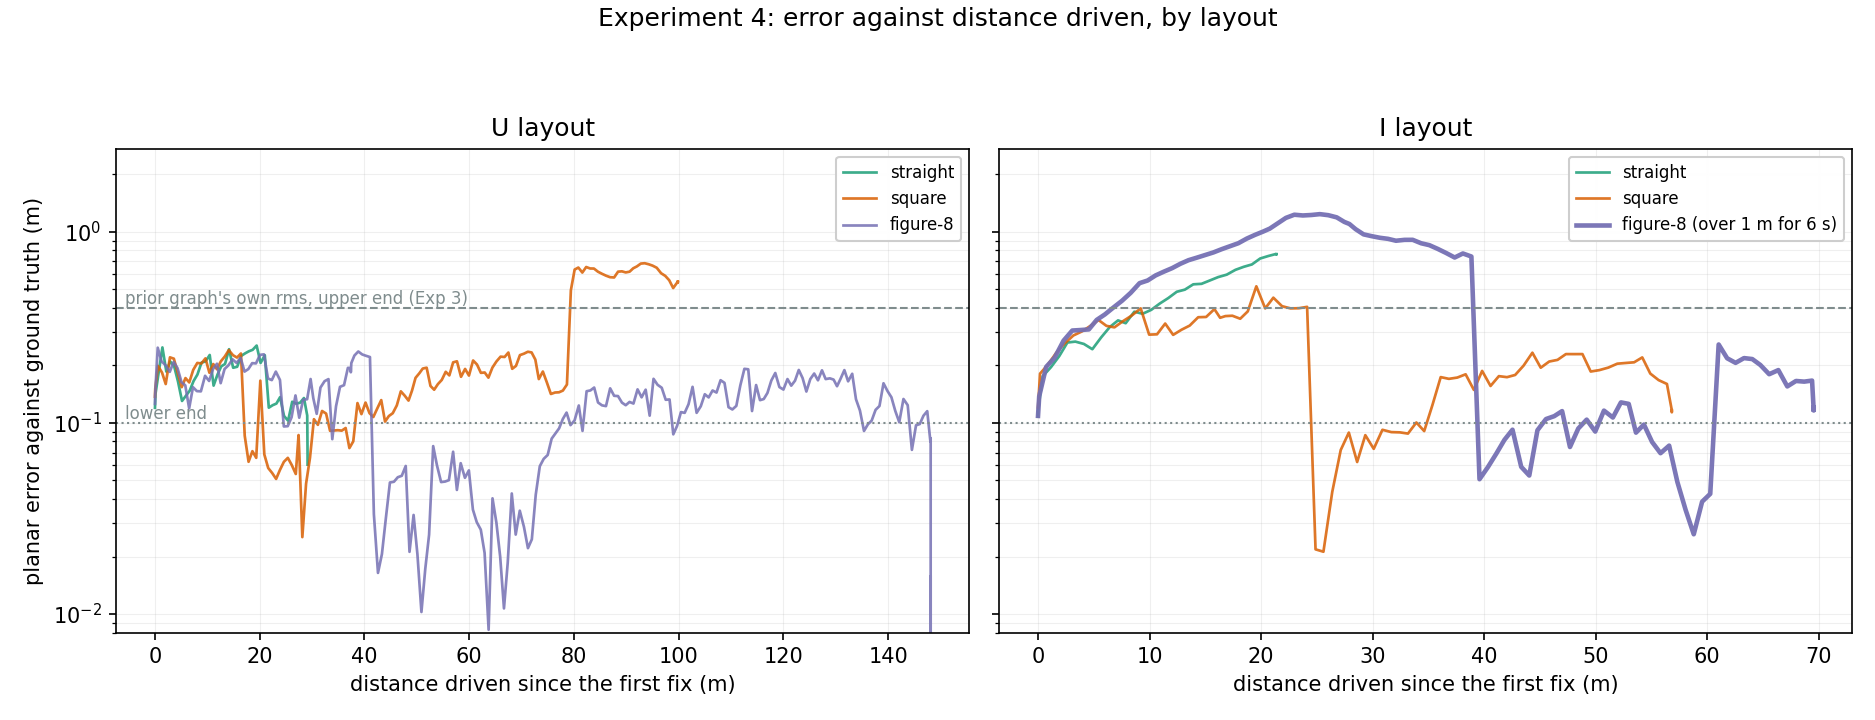
\includegraphics{exp4_error_vs_distance.png}}%
  {6 hand-driven runs, gate 1.5\,m: median error \textbf{0.13--0.21\,m},
   bounded in 5 of 6. One run over 1\,m for 6.5\,s, then back. Unaided ORB:
   the prior wins on all 4 routes $\ge$\,57\,m, loses the two shortest.}%
  {RTAB-9 can only match the map: graph 0.10--0.40\,m $\Rightarrow$ pose
   0.13--0.21\,m (\R{12}{}). The excursion is the gate's signature: a refused
   correction freezes map$\rightarrow$odom, the pose coasts on ORB odometry
   (ramp), then a fix is accepted (drop).}%
  {no repeats; a $\sim$0.1\,s timebase mismatch makes every figure an upper bound. Heading is worse on the I layout (1.3--2.8$^\circ$ vs 0.2--0.5$^\circ$), cause open.}
\end{frame}

% ---------------------------------------------------------------- R14
\begin{frame}[label=R14]{R14 \;What the results do not reach yet}
  \hl{NAV4}\hl{NAV5}\hl{NAV6}\hl{NAV7}\hl{NAV8}\navstrip\par\vspace{0.5em}
  \small
  \begin{itemize}\setlength{\itemsep}{0.35em}
    \item \textbf{NAV-4 \ldots\ NAV-8:} no goal was commanded in Experiment 4 (routes driven by
      hand), so the planner, controller and behaviour tree have no result. The open question
      from \R{12}{}: does a 3.8--10.2\,\% false-obstacle map block a route?
    \item \textbf{NAV-4 obstacle layer:} off in every run, so nothing tests a person in front of the robot.
    \item \textbf{Traffic in Experiment 4:} neither dynamic world was sampled.
    \item \textbf{VINS-3, 5, 6 and RTAB-4, 7:} no finding traced to them.
    \item \textbf{YOLO mask (Experiment 2):} it covers under a third of the moving pallet jacks'
      frames and none of the people, so the filtered arms are not reported.
  \end{itemize}
\end{frame}
